\documentclass{article}
\usepackage{float,amsmath}
\usepackage{graphicx}
\usepackage{color}
\usepackage[letterpaper,margin=1in]{geometry}
\usepackage{hyperref}

\usepackage{outlines}
\usepackage{enumitem}
\setenumerate[1]{label=\arabic*.}
\setenumerate[2]{label=\alph*.}
\setenumerate[3]{label=\arabic*.}
\setenumerate[4]{label=\roman*.}

\begin{document}

\author{HERA Team}
\title{HERA Rollout Plan}
\maketitle

\setcounter{section}{-1}
\section{Introduction}
The rollout plan for HERA centers around four systems:
\begin{itemize}
\item infrastructure
\item antenna construction
\item deployment of new system architecture (node, correlator)
\item updated implementation within the real-time processor (RTP)
\end{itemize}

HERA is operated in ``seasons'' that are denoted by:

\begin{table}[H]
\caption{HERA Operating Seasons}
\begin{tabular}{p{0.5in} p{2.2in} p{3.5in}} \hline
{\bf H0C} & season which ended in March 2017 & used the first 19 antennas (with their slightly wonky feeds). \\ \hline
{\bf H1C} & season to begin September 2017 & start with 42 (with possible additional of some of the ``missing 9''), them moving up to about 100 elements with improved feed.\\ \hline
{\bf H2C} & season to begin August 2018 & about 200 elements with full new feed/analog signal path\\ \hline
{\bf H3C} & season to begin August 2019 & about 350 elements \\ \hline
\end{tabular}
\end{table}

\begin{figure}
\includegraphics[width=\textwidth]{highlevel_timeline.pdf} %under ProjectBook/Schedule
\caption{High-level rollout timeline.}
\end{figure}

\section{H1C}
H1C will extend from about 1 September 2017 - 1 April 2018, and comprise about 100 (1C) antennas by the end of calendar year 2017.

\subsection{Infrastructure}
Before the start of the observing season, the current container compound in the center of the cleared PAPER circle will be moved to the western edge.  This is required to get it out of the way of the rest of the HERA build, but means that the current PAPER cables only reach a portion of the antennas, which impacts this season (see below).  Additionally, the servers in the CMC up by the accommodation will be moved into the KAPB and the network reconfiguration will be implemented.

\subsection{Antenna Construction}
The rollout of antennas is governed by our ability to construct them at pace and the constraint of using the existing cable-based architecture.  Note that of the 35 antennas currently built, nine of them are outside of the reachable radius with the cables (although some additional longer cables may be found and bring some of those back into operation).

\begin{figure}
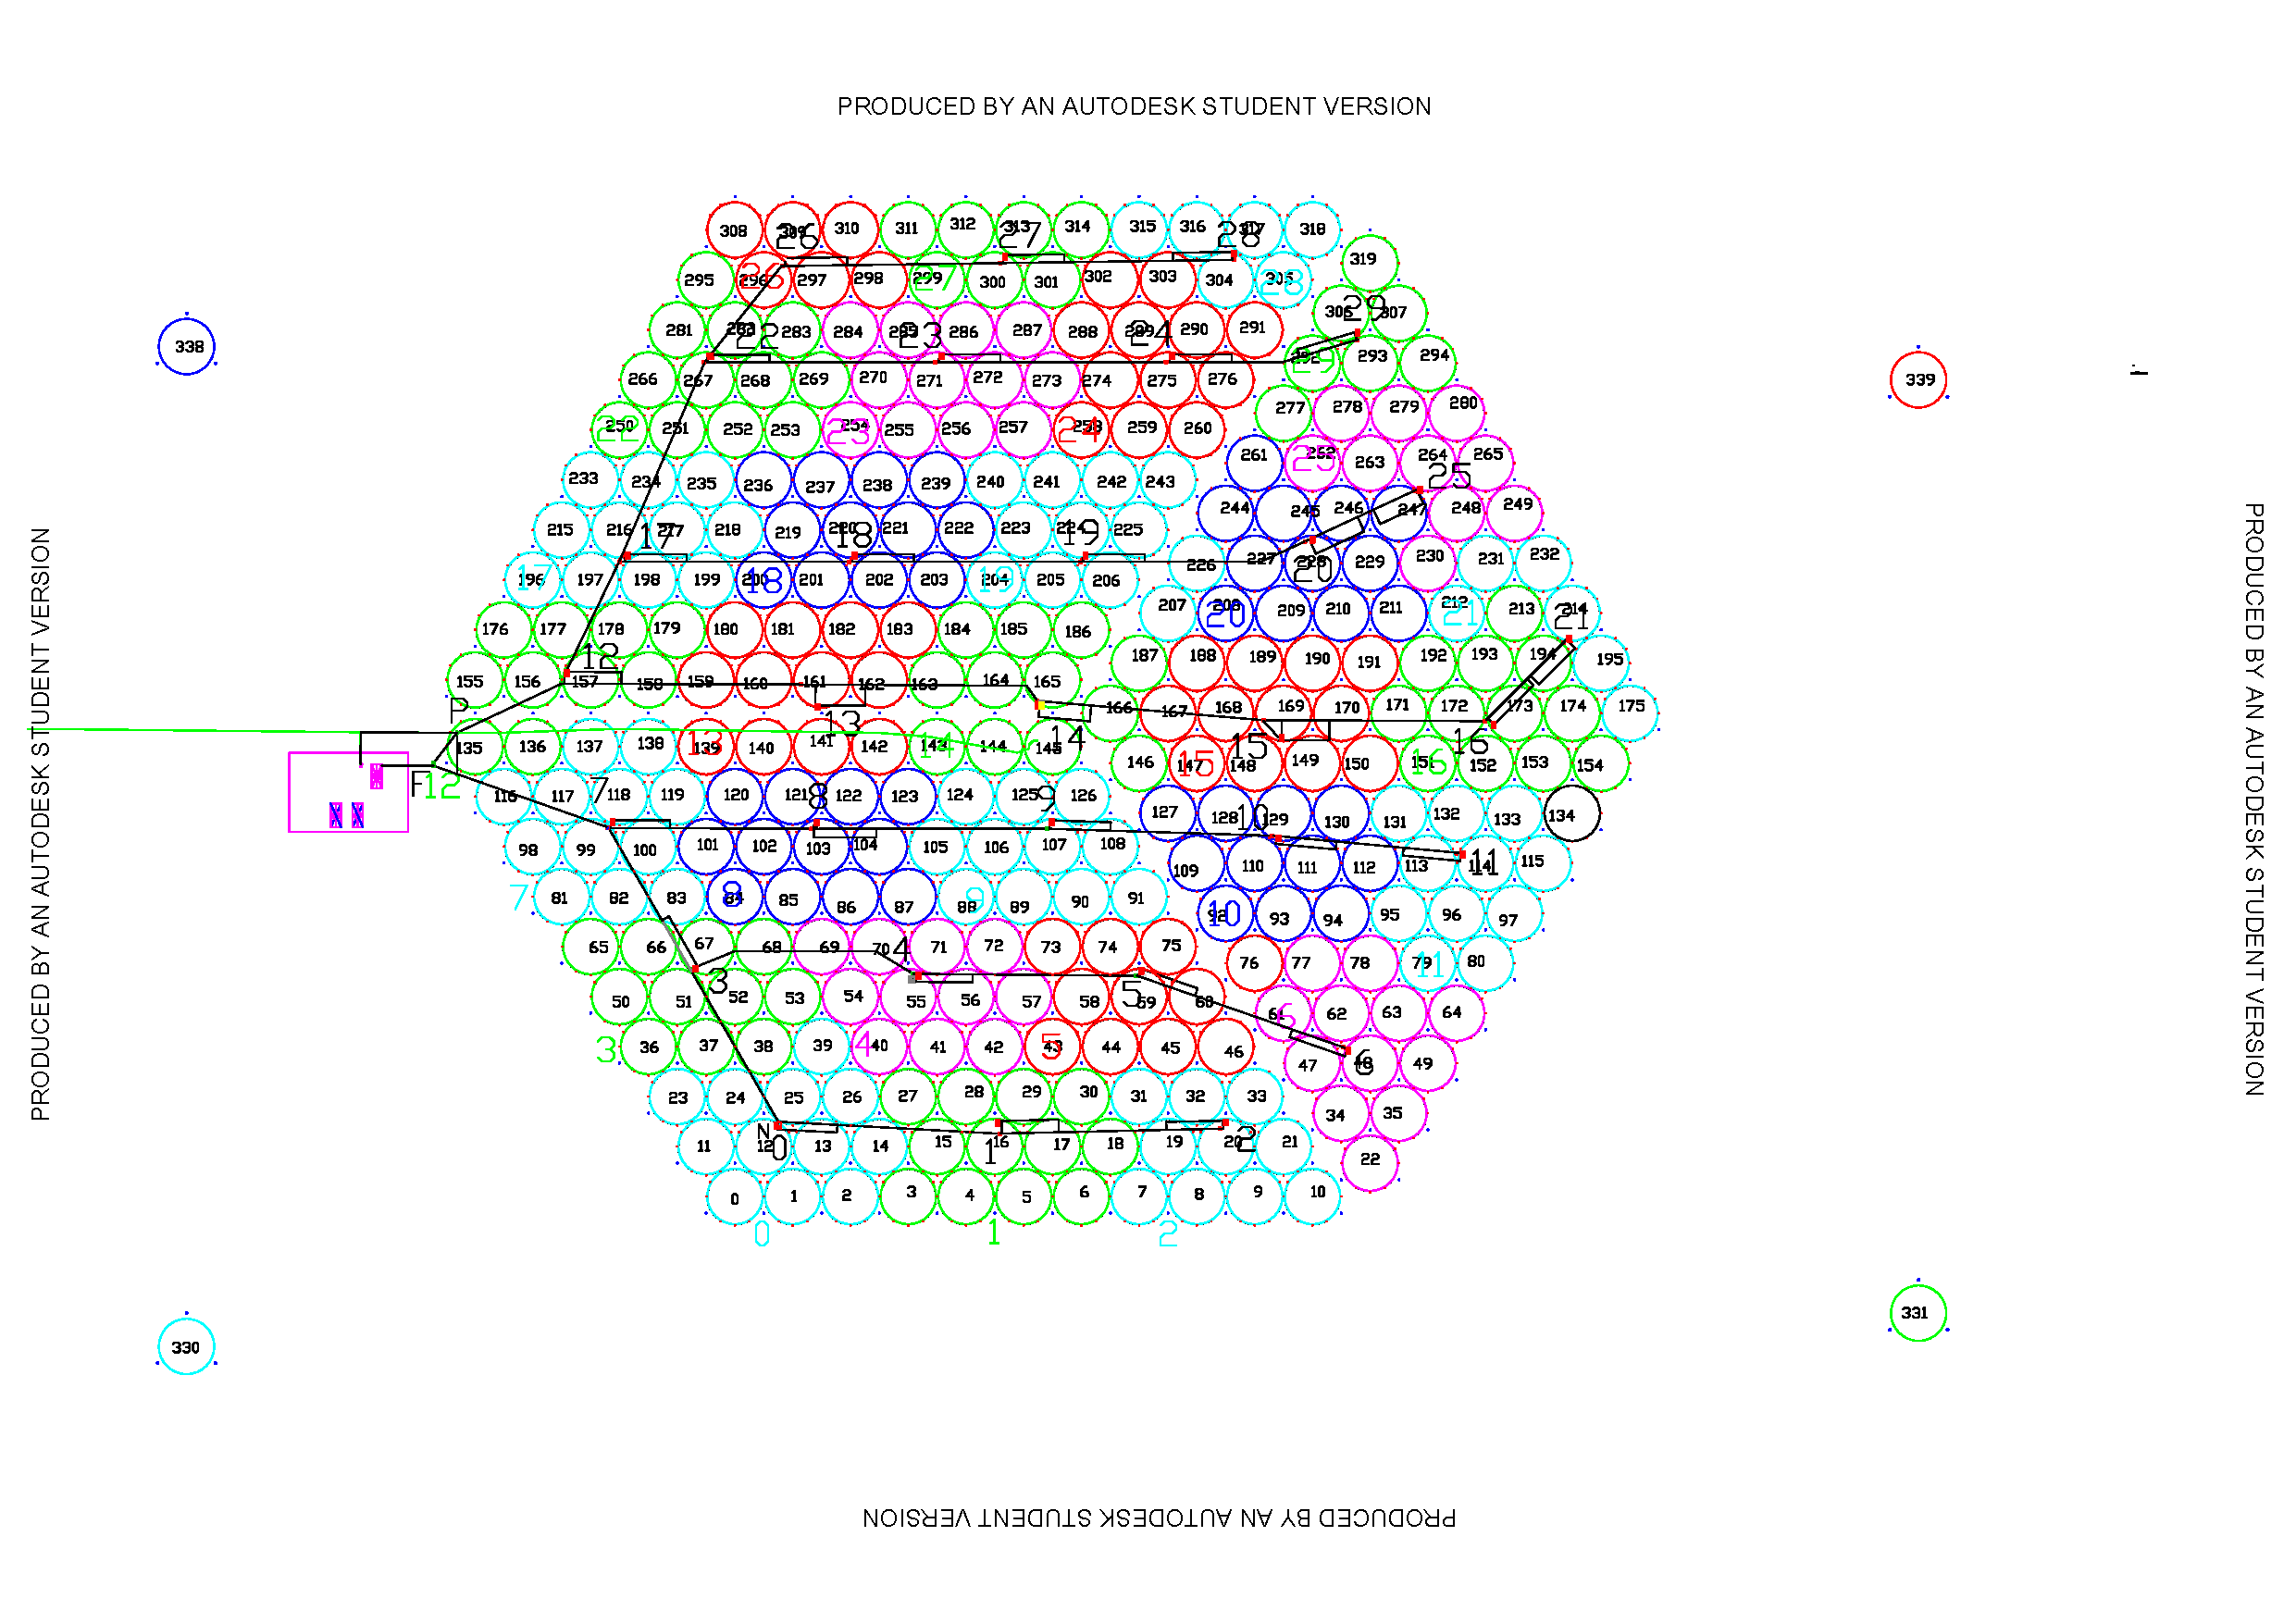
\includegraphics[width=\textwidth]{heraSite.pdf} %photoshopped version from design/hera-cad/heraSite.dwg; updated in that directory
\caption{H1C antenna rollout.}
\end{figure}

\subsection{System}

\subsection{RTP}


\section{H2C}
H1C will extend from about 1 September 2017 - 1 April 2018, and comprise about 100 (1C) antennas by the end of calendar year 2017.

\subsection{Infrastructure}

\subsection{Antenna Construction}

\subsection{System}

\subsection{RTP}

\section{H3C}
H1C will extend from about 1 September 2017 - 1 April 2018, and comprise about 100 (1C) antennas by the end of calendar year 2017.

\subsection{Infrastructure}

\subsection{Antenna Construction}

\subsection{System}

\subsection{RTP}

\end{document}
